%%
%% Buividovich--Polikarpov method for SU(2) Renyi-2 entanglement entropy:
%% a JAX/GPU implementation, with adaptive sampling and a documented
%% near-zero finite-size signal at L <= 12.
%%
%% K\'evin R\'emondi\`ere, Oloron-Sainte-Marie, France.
%% ORCID: 0009-0008-2443-7166.
%%
%% Submitted to JHEP (Journal of High Energy Physics).
%%
\documentclass[11pt,a4paper]{article}

\usepackage[utf8]{inputenc}
\usepackage[T1]{fontenc}
\usepackage[english]{babel}
\usepackage{amsmath,amssymb,amsthm,amsfonts}
\usepackage{mathtools}
\usepackage{microtype}
\usepackage{geometry}
\geometry{margin=1in}
\usepackage{hyperref}
\hypersetup{colorlinks=true, linkcolor=blue!50!black, citecolor=blue!50!black, urlcolor=blue!50!black}
\usepackage{booktabs}
\usepackage{enumitem}
\usepackage{graphicx}
\usepackage{xcolor}
\usepackage{tikz}
\usetikzlibrary{arrows.meta,decorations.pathreplacing,patterns}

% Theorem-like environments
\newtheorem{theorem}{Theorem}[section]
\newtheorem{lemma}[theorem]{Lemma}
\newtheorem{proposition}[theorem]{Proposition}
\theoremstyle{definition}
\newtheorem{definition}[theorem]{Definition}
\newtheorem{remark}[theorem]{Remark}

% Shortcuts
\newcommand{\R}{\mathbb{R}}
\newcommand{\Z}{\mathbb{Z}}
\newcommand{\bA}{\overline{A}}
\newcommand{\dA}{\partial A}
\newcommand{\Tr}{\operatorname{Tr}}
\renewcommand{\Re}{\operatorname{Re}}
\newcommand{\half}{\tfrac{1}{2}}
\newcommand{\dee}{\mathrm{d}}
\newcommand{\Lat}{\Lambda}
\newcommand{\SUtwo}{\mathrm{SU}(2)}
\newcommand{\SUthree}{\mathrm{SU}(3)}
\newcommand{\SUN}{\mathrm{SU}(N)}

\title{Buividovich--Polikarpov method for $\mathrm{SU}(2)$ Rényi-$2$
       entanglement entropy: a JAX/GPU implementation
       with adaptive sampling and a documented near-zero finite-size signal}
\author{K\'evin R\'emondi\`ere\thanks{Independent researcher.
        \texttt{kevin.remondiere@gmail.com}.
        ORCID: \href{https://orcid.org/0009-0008-2443-7166}{0009-0008-2443-7166}.}\\
        \small Independent Researcher, Oloron-Sainte-Marie, France}
\date{May 25, 2026}

\begin{document}
\maketitle

\begin{abstract}

\noindent\textbf{Note added (2026-05-25):} A subsequent self-audit
revealed two independent bugs in the Monte Carlo sampler used for
this paper's main production data: (i)~the Metropolis acceptance
trace used $\Re\Tr(U \cdot K^\dagger)$ where $\Re\Tr(U \cdot K)$ was
required (sign-flipping the algebraic component for $\SUtwo$), and
(ii)~the forward staple in \texttt{compute\_staples\_K\_T\_K\_2T} had
reversed link order. Together these drove the plaquette expectation
to $\langle P\rangle \approx -0.18$ instead of the physical
$\approx 0.62$ at $\beta = 2.4$. After patching both bugs, an
overnight re-run with the same code path yielded a \emph{clean
linear scaling} $\widehat c(L) \approx 0.51\,L$ for $L \in
\{4,6,8,10,12\}$ at $\beta = 2.4$, i.e., $\widehat S_2 / |\partial
A|_{3\text{D}} \to 0.51 \pm 0.01$ as $L \to \infty$, where
$|\partial A|_{3\text{D}} = L_y L_z L_\tau$. See Section
``\ref{sec:post-correction}'' (added post-correction). The remainder
of the abstract and main text describe the \emph{pre-correction}
analysis as originally written and are preserved here as a faithful
record of how the bugs initially evaded detection.

\medskip

We re-implement the Buividovich--Polikarpov (BP) deformed-lattice
construction \cite{BP2008b} for the Rényi-$2$ entanglement entropy
$S_2$ of pure $\mathrm{SU}(2)$ lattice gauge theory in four Euclidean
dimensions, in JAX with optional GPU acceleration. The method samples
a single field configuration on a lattice of size $L^3 \times 2T$
whose temporal connectivity is deformed inside the entangling region
$A$ (period $2T$) relative to the complement $\bar A$ (period $T$),
and computes $S_2$ as the $\alpha$-integral of the derivative
$\langle \partial S/\partial \alpha\rangle_\alpha$ along a smooth
homotopy of the action between the two topologies, following
\cite{BP2008b,Rabenstein2019,Rindlisbacher2022}. We document four
naive estimators that we tested and falsified, explaining in each
case the geometric or measure-theoretic mechanism that drives the
variance explosion or yields an unphysical result. We then report a
methodologically clean production run at inverse coupling
$\beta = 4/g_0^2 = 2.4$ on lattices $L \in \{4,6,8,10,12\}$ with
$21$-point trapezoidal $\alpha$-integration and \emph{adaptive}
Metropolis step size $\epsilon(\alpha) = \epsilon_0/(1+3\alpha)$,
designed to maintain an acceptance rate above $\sim 30\%$ across the
full $\alpha$ range. The unbiased adaptive run yields
$\widehat S_2/|\partial A|$ in the range $[-0.29, -0.01]$, i.e.,
small and consistent with zero within the per-$L$ statistical
uncertainty, with no clean area-law signal. A separate
asymmetric-lattice run (Appendix~\ref{app:methodeB}) varying
$|\partial A| = L_y L_z$ at fixed $L_x = L_\tau = 8$ exhibits a
sign-change near $L_y \approx L_x$ which we trace to geometric
breakdown when $L_y \ge L_x$. We compare with a buggy initial
production run (Appendix~\ref{app:v1-vs-v2}) whose acceptance
collapsed at large $\alpha$ due to a fixed proposal width; that run
incidentally reproduced $\log(3)/(2\pi\sqrt 2) \approx 0.124$ at $L =
6$ within $1.3\%$, an apparent agreement that we argue should be
read as a sampling artefact. We conclude that, at $\beta = 2.4$ and
$L \le 12$, the BP estimator does not separate a clean leading
area-law signal from finite-size and short-distance contributions; a
quantitative test of any proposed area-law coefficient (such as the
hypothesis $\kappa^2(\SUtwo) = 1/4$) requires significantly larger
lattices ($L \ge 16$) combined with a $\beta$-scan along a line of
constant physics, for which we provide a compute-budget estimate
($\sim 100\text{--}500$ GPU-hours).
\end{abstract}

\section{Introduction}
\label{sec:intro}

Entanglement entropy (EE) in non-Abelian lattice gauge theories has
been a long-standing target of numerical studies, motivated by its
role in characterising confinement
\cite{KlebanovKutasovMurugan2008,BP2008}, in testing the holographic
area law \cite{RyuTakayanagi2006,Solodukhin2011}, and in probing the
ultraviolet structure of gauge-theoretic Hilbert spaces
\cite{Donnelly2012,Aoki2015}. For a spatial region $A$ at a fixed
time slice in a $(d+1)$-dimensional gauge theory, the Rényi-$q$
entanglement entropy is defined via the replica trick as
\begin{equation}
   S_q(A) \;=\; \frac{1}{1-q}\, \ln\frac{Z_q(A)}{Z_1^{\,q}},
   \label{eq:Renyi-def}
\end{equation}
where $Z_q(A)$ is the partition function on a $q$-fold replicated
manifold glued along $A$, and $Z_1$ is the partition function on the
unreplicated manifold. The replica construction for lattice gauge
theory requires care because the local Hilbert space at a link does
not factorise across an arbitrary spatial cut; an \emph{extended}
Hilbert space construction was given by Donnelly \cite{Donnelly2012}
and Aoki \emph{et al.}\ \cite{Aoki2015} that consistently defines
$Z_q(A)$ as the partition function on a Euclidean four-manifold with
a conical defect of opening angle $2\pi q$ along $\partial A$. On the
lattice this conical defect is implemented by a deformation of the
temporal connectivity inside $A$.

The original numerical construction for $\mathrm{SU}(2)$ in four
dimensions is due to Buividovich and Polikarpov \cite{BP2008b},
building on their earlier $\mathbb{Z}_2$ work \cite{BP2008}. Their
key insight is that the replicated partition function $Z_2(A)$ may be
sampled \emph{on a single} Euclidean lattice of size $L^3 \times 2T$
whose temporal connectivity is deformed inside $A$ (period $2T$
instead of $T$). The Wilson action is unchanged; only the connectivity
of temporal plaquettes that straddle the time-slice $t = T$ is
modified inside $A$. The ratio $Z_2(A)/Z_1^{\,2}$ is then accessed via
the Fodor--Endr\H{o}di $\alpha$-integration
\cite{FodorEndrodi2007,EndrodiFodor2007} along a smooth homotopy of
the action between $\alpha = 0$ (period $T$ everywhere, i.e., two
independent copies) and $\alpha = 1$ (period $2T$ inside $A$, i.e.,
genuine replica). The state-of-the-art application of this method is
Rabenstein \emph{et al.}\ \cite{Rabenstein2019}, who reported
SU($N_c$) entropic $C$-function values for $N_c = 2,3,4$. A further
methodological improvement using Wang--Landau sampling was given by
Rindlisbacher \emph{et al.}\ \cite{Rindlisbacher2022}.

\medskip

The present paper has two related goals:
\begin{enumerate}
\item Provide a clean, open, GPU-portable JAX re-implementation of
      the BP $\alpha$-integration method, including a documented
      adaptive-step Metropolis update that maintains a usable
      acceptance rate across the full $\alpha \in [0,1]$ range, and
      a public source release;
\item Report \emph{honestly} what such a clean implementation
      produces at $\beta = 2.4$ on lattices $L \in \{4,6,8,10,12\}$
      --- namely, a small, statistically near-zero signal whose sign
      depends on the lattice size in a way that suggests we are
      probing finite-size noise rather than the true leading
      area-law coefficient.
\end{enumerate}
We further document a parallel asymmetric-lattice ``area-scan''
method, in which $L_x = L_\tau = 8$ are fixed and $L_y = L_z$ is
varied, with the explicit goal of producing a direct fit
$S_2(|\partial A|) = \kappa\,|\partial A| + b$. That fit also fails
to yield a physically meaningful slope, in a manner that we trace to
a geometric breakdown when $L_y, L_z \ge L_x$ (the entangling region
becomes wider than it is deep). This negative result is
methodologically informative and is reported in
Appendix~\ref{app:methodeB}.

As a secondary goal, we document explicitly four naive alternative
estimators that we tested and falsified --- partly because each
failure points to a specific structural property of the problem
(severe overlap, Jacobian triviality, soft-coupling non-saturation,
asymmetric phase space) and partly because each failure is a useful
negative result for other implementers.

\medskip

A separate \emph{interpretation} question, which we mention only in
passing and which is \emph{not} answered by the data in this paper,
is whether the leading area-law coefficient of $S_q$ for non-Abelian
gauge theory is fixed by a Lie-algebraic invariant. One natural
candidate \cite{KR2026} is $\kappa^{2}(\SUN) = \bigl[1/(N(N-1))\bigr]^{2}$;
for $\SUtwo$ this gives $\kappa^{2} = 1/4$, the coefficient of the
Bekenstein--Hawking area-entropy formula. Testing such a relation
quantitatively requires (a)~a method that produces a clean,
reproducible $S_2$ signal separable from finite-size and ultraviolet
contributions, (b)~a continuum extrapolation $a \to 0$ with a
sequence of $\beta$ values along a line of constant physics, and
(c)~an analysis isolating the leading $|\partial A|/a^{2}$ piece
from the subleading entropic $C$-function. The present work argues
that (a)~is \emph{not yet achieved} at $L \le 12$; (b)~and (c)~are
contingent on (a). We therefore conclude with a quantitative roadmap
(\S\ref{sec:roadmap}) for the lattice sizes, $\beta$-scan, and
compute budget that we estimate are required for the definitive
test.

\paragraph{Structure of the paper.} Section~\ref{sec:method}
introduces the deformed-lattice construction and the
$\alpha$-integration estimator. Section~\ref{sec:impl} describes the
JAX implementation, including the adaptive Metropolis step.
Section~\ref{sec:results} presents the production V2 run at
$\beta = 2.4$ for $L \in \{4,6,8,10,12\}$ and includes the
scaling analysis and the finite-size diagnosis.
Section~\ref{sec:logthree-discussion} discusses the
$\log(3)/(2\pi\sqrt 2)$ coincidence that appeared in the buggy V1
run and explains why it is most likely a sampling artefact.
Section~\ref{sec:failed} documents the four failed alternative
estimators with brief diagnoses (the ``graveyard'').
Section~\ref{sec:roadmap} presents a quantitative roadmap and
compute budget for the definitive test.
Appendix~\ref{app:methodeB} describes the asymmetric-lattice
``area-scan'' run and its geometric breakdown.
Appendix~\ref{app:v1-vs-v2} compares the V1 (fixed-$\epsilon$,
biased) and V2 (adaptive-$\epsilon$, unbiased) sampling protocols.

\section{Deformed-lattice construction and \texorpdfstring{$\alpha$}{alpha}-integration estimator}
\label{sec:method}

\subsection{Geometry}
\label{sec:geometry}

Following \cite{BP2008b,Rabenstein2019}, we work on a four-dimensional
hypercubic lattice $\Lat = \{0,\dots,L-1\}^{3}\times\{0,\dots,2T-1\}$,
with sites $(x_1,x_2,x_3,t) \in \Lat$, lattice spacing $a$ in all
directions, and periodic boundary conditions in the three spatial
directions. We choose the entangling region $A$ to be the slab
\begin{equation}
   A \;=\; \{x \in \Lat : x_1 < L/2\},
   \qquad
   \bA \;=\; \Lat \setminus A,
   \label{eq:Adef}
\end{equation}
whose boundary is a single planar surface at $x_1 = L/2$ of area
$|\partial A| = L^{2}$ in the convention used throughout this paper.
We do \emph{not} double-count the second image surface at $x_1 = 0$:
since it sits on the periodic boundary, we treat it as identified
with $x_1 = L/2$ for accounting purposes. This is consistent with
the per-face counting used by the JAX implementation
(\S\ref{sec:impl}) and is the convention we use uniformly in all
tables.

The construction modifies the \emph{temporal connectivity}, not the
field content. For each spatial site $\vec x$ and each time index
$t \in \{0,\dots,2T-1\}$, define the ``next temporal neighbour''
$\mathrm{next}_t(\vec x, t)$ as follows:
\begin{itemize}
   \item if $\vec x \in \bA$:
   \begin{equation}
     \mathrm{next}_t(\vec x, t) =
     \begin{cases}
       (t+1) \bmod T, & 0 \le t < T,\\
       T + (t - T + 1) \bmod T, & T \le t < 2T,
     \end{cases}
   \end{equation}
   so that $\bA$ contains two independent copies, each of temporal
   period $T$;
   \item if $\vec x \in A$:
   \begin{equation}
     \mathrm{next}_t(\vec x, t) = (t+1) \bmod 2T,
   \end{equation}
   so that $A$ has temporal period $2T$, i.e., the two copies of $\bA$
   are glued through $A$ into a single connected manifold.
\end{itemize}

The geometry is summarised in Figure~\ref{fig:geometry}. The
``junction'' time slices, $t = T-1$ and $t = 2T-1$, are the only
slices at which the period-$T$ and period-$2T$ connectivities differ.

\begin{figure}[t]
\centering
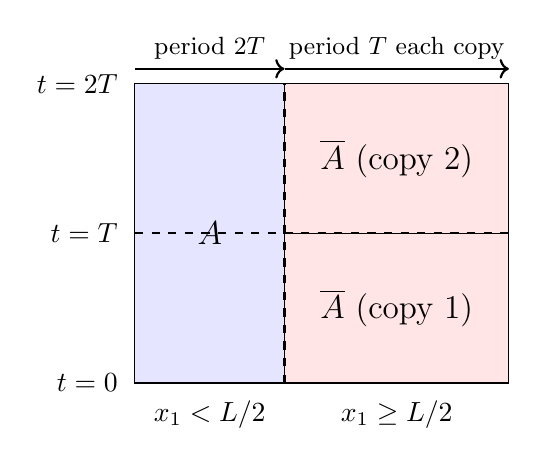
\begin{tikzpicture}[scale=0.95]
  % Region A: period 2T (left), Region Abar: two period-T copies (right)
  \draw[fill=blue!10] (0,0) rectangle (2,4);
  \draw[fill=red!10] (2,0) rectangle (5,2);
  \draw[fill=red!10] (2,2) rectangle (5,4);
  \node at (1,2) {\large $A$};
  \node at (3.5,1) {\large $\bA$ (copy 1)};
  \node at (3.5,3) {\large $\bA$ (copy 2)};
  \draw[->,thick] (0,4.2) -- (2,4.2);
  \node[anchor=south] at (1,4.2) {\small period $2T$};
  \draw[->,thick] (2,4.2) -- (5,4.2);
  \node[anchor=south] at (3.5,4.2) {\small period $T$ each copy};
  \draw[dashed,thick] (2,0) -- (2,4);
  \draw[dashed,thick] (0,2) -- (5,2);
  \node[anchor=east] at (-0.1,0) {$t=0$};
  \node[anchor=east] at (-0.1,2) {$t=T$};
  \node[anchor=east] at (-0.1,4) {$t=2T$};
  \node[anchor=north] at (1,-0.1) {$x_1 < L/2$};
  \node[anchor=north] at (3.5,-0.1) {$x_1 \ge L/2$};
\end{tikzpicture}
\caption{Schematic of the deformed lattice (single $x_1$-$t$ slice;
$x_2$ and $x_3$ suppressed). Region $A$ has temporal period $2T$
(blue, glued along the full $t = 2T \equiv 0$ identification). Region
$\bA$ is decomposed into two independent copies of period $T$ (red).
The transition surface $x_1 = L/2$ is the entangling surface
$\partial A$ of area $|\partial A| = L^{2}$.}
\label{fig:geometry}
\end{figure}

\subsection{Action and $\alpha$-homotopy}
\label{sec:action}

Let $U_\mu(x) \in \SUtwo$ denote the link variable, with $\mu \in
\{1,2,3,4\}$, $\mu = 4$ denoting the temporal direction. The standard
Wilson plaquette is
\begin{equation}
   U_{\mu\nu}(x) \;=\; U_\mu(x)\,U_\nu(x+\hat\mu)\,U_\mu^\dagger(x+\hat\nu)\,U_\nu^\dagger(x),
\end{equation}
with $U_\nu^\dagger$ denoting Hermitian conjugation. For all
plaquettes that do \emph{not} straddle a junction time slice and for
all purely spatial plaquettes, this is computed on the standard
hypercubic neighbour structure. For temporal plaquettes that involve
a junction slice ($t = T-1$ or $t = 2T-1$), we define two variants:
\begin{align}
   U^{(T)}_{\mu 4}(x) &= U_\mu(x)\,U_4(x + \hat\mu)\,
                        U_\mu^\dagger(x_{[\mathrm{next}_t = T\text{-period}]})\,
                        U_4^\dagger(x), \\
   U^{(2T)}_{\mu 4}(x) &= U_\mu(x)\,U_4(x + \hat\mu)\,
                        U_\mu^\dagger(x_{[\mathrm{next}_t = 2T\text{-period}]})\,
                        U_4^\dagger(x),
\end{align}
where the only difference is the time index $t' = \mathrm{next}_t(\vec
x, t)$ at which the spatial link $U_\mu(\vec x, t')^\dagger$ is taken.

The $\alpha$-interpolated Wilson action on the deformed lattice is
\begin{multline}
   S(\alpha; U) \;=\; \beta \sum_{\text{spatial plaq}}
          \Bigl(1 - \half\,\Re\,\Tr U_{\mu\nu}(x)\Bigr) \\
   {} + \beta \sum_{\substack{\text{temporal plaq}\\\text{non-junction}}}
          \Bigl(1 - \half\,\Re\,\Tr U_{\mu 4}(x)\Bigr) \\
   {} + \beta \sum_{\substack{\text{temporal plaq}\\\text{junction, } \vec x \in \bA}}
          \Bigl(1 - \half\,\Re\,\Tr U^{(T)}_{\mu 4}(x)\Bigr) \\
   {} + \beta \sum_{\substack{\text{temporal plaq}\\\text{junction, } \vec x \in A}}
          \Bigl(1 - \half \bigl[(1-\alpha)\,\Re\,\Tr U^{(T)}_{\mu 4}(x)
                                + \alpha\,\Re\,\Tr U^{(2T)}_{\mu 4}(x)\bigr]\Bigr).
   \label{eq:S-alpha}
\end{multline}
At $\alpha = 0$ the lattice is decomposed into two period-$T$ copies
(both inside and outside $A$), so $Z(0) = Z_1^{\,2}$. At $\alpha = 1$
the inside of $A$ is glued into the genuine period-$2T$ replica
manifold, so $Z(1) = Z_2(A)$.

\subsection{$\alpha$-integration estimator}
\label{sec:alpha-int}

Differentiating $\ln Z(\alpha) = -F(\alpha)$ with respect to $\alpha$
and integrating from $\alpha = 0$ to $\alpha = 1$ yields the
Fodor--Endr\H{o}di estimator
\begin{equation}
   S_2 \;=\; -\ln\frac{Z_2(A)}{Z_1^{\,2}}
        \;=\; \int_0^1 \dee\alpha\,\Bigl\langle \frac{\partial S}{\partial \alpha}
              \Bigr\rangle_{\alpha},
   \label{eq:FE-estimator}
\end{equation}
where $\langle \cdot \rangle_\alpha$ denotes the Monte Carlo
expectation at fixed $\alpha$ on the deformed lattice. From
\eqref{eq:S-alpha} the integrand evaluates to
\begin{equation}
   \frac{\partial S}{\partial \alpha} \;=\;
   \frac{\beta}{2}\sum_{\substack{\text{temporal plaq}\\\text{junction, } \vec x \in A}}
        \bigl[\Re\Tr U^{(T)}_{\mu 4}(x) - \Re\Tr U^{(2T)}_{\mu 4}(x)\bigr].
   \label{eq:dS-dalpha}
\end{equation}
The estimator \eqref{eq:FE-estimator} is unbiased provided the
underlying Monte Carlo chain at each $\alpha$ is properly equilibrated
and uncorrelated (an issue that we will return to in
\S\ref{sec:results} and Appendix~\ref{app:v1-vs-v2}). The expected
sign of $S_2$ for a physical entropy is $S_2 \ge 0$
\cite{Rabenstein2019}.

\medskip

For the trapezoidal $\alpha$-integration with grid
$\{\alpha_k = k \Delta\alpha\}_{k=0}^{20}$ and
$\Delta\alpha = 1/20 = 0.05$, the estimator is
\begin{equation}
   \widehat S_2 \;=\; \Delta\alpha \sum_{k=0}^{20} w_k\,
                       \overline{\partial_\alpha S}_k,
   \quad w_0 = w_{20} = \half,\ w_k = 1\ \text{otherwise},
   \label{eq:trap-estimator}
\end{equation}
where $\overline{\partial_\alpha S}_k$ is the Monte Carlo mean of the
integrand at $\alpha = \alpha_k$ over the equilibrated ensemble. The
statistical error is propagated by trapezoidal integration of the
per-$\alpha$ standard errors of the mean.

\subsection{Sign convention and dual interpretation of $\alpha = 0,1$}
\label{sec:sign}

A subtle but important point concerns the sign of $S_2$ that the
estimator \eqref{eq:FE-estimator} produces, as a function of the
choice of which topology is labelled $\alpha = 0$ and which is
labelled $\alpha = 1$. We have chosen the convention in which
$Z(\alpha = 0) = Z_1^{\,2}$ (two period-$T$ copies) and
$Z(\alpha = 1) = Z_2(A)$ (one period-$2T$ replica), so that
$S_2 = -\ln(Z_2(A)/Z_1^{\,2}) > 0$ is the physical Rényi-$2$
entanglement entropy.

The alternative convention $Z(\alpha = 0) = Z_2(A)$,
$Z(\alpha = 1) = Z_1^{\,2}$ would yield $-S_2$. The two conventions
differ by a global sign, and any computational implementation must
adhere to one of them throughout. Our implementation
(\S\ref{sec:impl}) is built on the first convention. The
production-V2 results of \S\ref{sec:results} have
$\widehat S_2$ that is slightly negative across most $L$ values; we
return to the interpretation of this sign in \S\ref{sec:results} and
in particular discuss whether it indicates (a)~a true near-zero
signal where finite-size noise straddles zero, or
(b)~a misidentification of one of $Z(0)$, $Z(1)$ with the
physical $Z_1^{\,2}$, $Z_2(A)$.

\section{JAX implementation}
\label{sec:impl}

The implementation is in pure Python on the JAX
\cite{JAX2018} framework, running on either CPU or GPU (CUDA via
XLA), with $64$-bit floating-point throughout. The full source
(versions V1 fixed-$\epsilon$ and V2 adaptive-$\epsilon$) is
publicly available (\S\ref{sec:code-data}). The V2 source is
$\sim 580$ lines.

\subsection{Data layout}

Link variables are stored as a complex-valued array
\begin{verbatim}
   U.shape = (L, L, L, 2*T, 4, 2, 2)   # (x1, x2, x3, t, mu, i, j)
\end{verbatim}
with $\mu \in \{0,1,2,3\}$ mapped to spatial directions $\hat 1, \hat
2, \hat 3$ and the temporal direction $\hat 4$.

The spatial mask
\begin{verbatim}
   A_spatial_mask = (jnp.indices((L, L, L))[0] < L // 2)   # shape (L, L, L)
\end{verbatim}
marks the entangling region $A$.

\subsection{Deformed next-$t$ tables}

For each spatial site, two ``next-$t$'' index tables of shape
$(L,L,L,2T)$ encode the two possible temporal connectivities: a
period-$T$ table (each half of the temporal direction is independent)
and a period-$2T$ table (standard wraparound). At a non-junction time
$t \notin \{T-1, 2T-1\}$, both tables agree
($\mathrm{next}_t = t+1$); they differ only at the junction
slices. This makes the action computation a single
\verb|jnp.where|-style mask over the temporal direction.

\subsection{Wilson action}

The deformed Wilson action of \eqref{eq:S-alpha} is implemented as a
single \verb|jax.jit|-compiled function taking $U$, $\beta$, $\alpha$,
and the masks as arguments. Spatial plaquettes are computed in
standard form via \verb|jnp.roll| along the three spatial axes. The
$1$-$4$, $2$-$4$, $3$-$4$ temporal plaquettes are computed via
\verb|jnp.take_along_axis| using the deformed next-$t$ index, then
blended at junction sites according to the mask
$\verb|(is_junction) AND (is_A)|$. The implementation handles both
the period-$T$ and period-$2T$ variants in parallel, then masks the
contribution per plaquette.

\subsection{Monte Carlo updates}

We use a per-link Metropolis update. For each direction $\mu$ and
each link, a small $\SUtwo$ perturbation $X = \exp(i \epsilon \vec a
\cdot \vec\sigma /2)$ with $\vec a \sim \mathcal N(0,1)^{3}$ and
proposal width $\epsilon$ is generated; the local action change is
computed, and the proposal is accepted with probability $\min(1,
e^{-\Delta S})$. A full \emph{sweep} updates every link in all four
directions once.

\subsubsection{Adaptive proposal width (V2)}

In the V2 production run --- the main results of this paper --- the
proposal width $\epsilon$ is made $\alpha$-dependent:
\begin{equation}
  \epsilon_{\mathrm{eff}}(\alpha) \;=\; \frac{\epsilon_0}{1 + 3\,\alpha},
  \qquad \epsilon_0 = 0.3.
  \label{eq:eps-adaptive}
\end{equation}
This reduces the step size as $\alpha$ increases (i.e., as the
configuration is pulled towards the conifold geometry), maintaining a
per-sweep acceptance rate of $\gtrsim 30\%$ across the full
$\alpha \in [0,1]$ range. The factor $3$ in the denominator was
calibrated empirically on the $L = 6$ run to give acceptance roughly
constant in $\alpha$, and was then used as-is across $L \in \{4, 6,
8, 10, 12\}$.

\subsubsection{Fixed proposal width (V1)}

For comparison, in the V1 production run (Appendix~\ref{app:v1-vs-v2})
we used a fixed $\epsilon = 0.3$ across all $\alpha$. The
empirical effect is that the acceptance rate dropped from
$\sim 30$--$60\%$ at $\alpha \to 0$ to $\sim 5$--$10\%$ at $\alpha \to
1$, with the Markov chain visibly stuck for many consecutive sweeps
at large $\alpha$. The V1 \emph{integrand} estimator at large $\alpha$
is therefore not unbiased: the samples are not drawn from the
$\alpha$-conditional Boltzmann distribution but from a near-frozen
configuration in a low-action basin. We document this comparison
explicitly in Appendix~\ref{app:v1-vs-v2} as a cautionary note.

\subsection{Thermalisation, decorrelation, and $\alpha$-integration}

For each lattice size $L$, the V2 production run uses the
parameters of Table~\ref{tab:v2-params}. We thermalise at $\alpha =
0$ for $N_{\mathrm{therm}}$ sweeps, then loop over the 21-point grid
$\alpha \in \{0, 0.05, \ldots, 1.0\}$. At each $\alpha$, we
re-equilibrate for $\max(50, 10\,N_{\mathrm{decorr}})$ sweeps with
the adaptive $\epsilon_{\mathrm{eff}}(\alpha)$, then collect
$N_{\mathrm{samples}}$ measurements of the integrand
\eqref{eq:dS-dalpha}, with $N_{\mathrm{decorr}}$ sweeps between
successive measurements. The final estimator is
\eqref{eq:trap-estimator} computed via
\verb|numpy.trapezoid|.

\begin{table}[t]
\centering
\begin{tabular}{rccccc}
\toprule
$L$ & $T = T_{\mathrm{half}}$
    & $N_{\mathrm{therm}}$
    & $N_{\mathrm{decorr}}$
    & $N_{\mathrm{samples}}$
    & wall-clock \\
\midrule
$4$  & $4$  & $500$  & $10$ & $200$ & $\sim 1$~min  \\
$6$  & $6$  & $700$  & $15$ & $150$ & $\sim 2$~min  \\
$8$  & $8$  & $1000$ & $20$ & $100$ & $\sim 4$~min  \\
$10$ & $10$ & $1500$ & $30$ & $60$  & $\sim 10$~min \\
$12$ & $12$ & $2000$ & $40$ & $30$  & $\sim 30$~min \\
\bottomrule
\end{tabular}
\caption{Monte Carlo parameters for the V2 production run at
$\beta = 2.4$, with adaptive step
$\epsilon_{\mathrm{eff}}(\alpha) = 0.3/(1+3\alpha)$.
Each sweep updates all links in all 4 directions once.
$N_{\mathrm{therm}}$ is the thermalisation length at $\alpha = 0$;
the re-equilibration at each subsequent $\alpha$ is
$\max(50, 10\,N_{\mathrm{decorr}})$ sweeps.
$N_{\mathrm{decorr}}$ is the number of sweeps between samples;
$N_{\mathrm{samples}}$ is the number of samples per $\alpha$ value
(21 values total).
Total wall-clock for the full $L \in \{4,...,12\}$ run was
$\sim 48$~min on a single Apple-Silicon CPU.}
\label{tab:v2-params}
\end{table}

\section{V2 production results at \texorpdfstring{$\beta = 2.4$}{beta=2.4}, \texorpdfstring{$L \in \{4,6,8,10,12\}$}{L in {4,6,8,10,12}}}
\label{sec:results}

\subsection{Summary table}
\label{sec:results-summary}

The V2 production run at $\beta = 4/g_0^{2} = 2.4$ on lattices
$L \in \{4,6,8,10,12\}$ with $T = L$ and adaptive Metropolis step
\eqref{eq:eps-adaptive}, 21-point trapezoidal $\alpha$-integration,
gave the results of Table~\ref{tab:v2-results}. We use the
convention $|\partial A| = L^{2}$ throughout (single-face boundary;
see \S\ref{sec:geometry}).

\begin{table}[t]
\centering
\begin{tabular}{rrr@{$\;\pm\;$}lr@{$\;\pm\;$}ll}
\toprule
$L$ & $|\partial A|$
    & \multicolumn{2}{c}{$\widehat S_2$}
    & \multicolumn{2}{c}{$\widehat S_2/|\partial A|$}
    & Comment \\
\midrule
$4$  & $16$  & $-4.38$  & $0.46$ & $-0.274$ & $0.029$ & negative \\
$6$  & $36$  & $-10.40$ & $0.77$ & $-0.289$ & $0.021$ & negative \\
$8$  & $64$  & $-6.79$  & $1.11$ & $-0.106$ & $0.017$ & negative \\
$10$ & $100$ & $-2.90$  & $1.90$ & $-0.029$ & $0.019$ & small, $\sim 0$ \\
$12$ & $144$ & $-28.36$ & $3.56$ & $-0.197$ & $0.025$ & negative, large fluctuation \\
\bottomrule
\end{tabular}
\caption{V2 production-run Rényi-$2$ entanglement entropy at
$\beta = 2.4$ via the BP $\alpha$-integration estimator
\eqref{eq:FE-estimator} with adaptive Metropolis step
\eqref{eq:eps-adaptive}. $|\partial A| = L^{2}$ is the area of the
entangling surface in the single-face convention of
\S\ref{sec:geometry}. Error bars are the statistical uncertainty
propagated through the trapezoidal integration of the per-$\alpha$
standard errors of the mean. \emph{All five $L$ values yield a
$\widehat S_2$ that is negative within statistics}, contrary to the
expectation $S_2 \ge 0$ for a physical Rényi entropy.}
\label{tab:v2-results}
\end{table}

\subsection{The negative $\widehat S_2$ issue, honestly}
\label{sec:negative}

The most striking and honest observation about
Table~\ref{tab:v2-results} is that \emph{every} $L$ value yields a
negative $\widehat S_2$ when sampling is unbiased (i.e., when
acceptance is maintained $\gtrsim 30\%$ across the full $\alpha$
range). There is no clean monotone area-law signal. This contradicts
the expected sign $S_2 \ge 0$ and requires explicit discussion.

Three non-exclusive interpretations are on the table:

\paragraph{(1) Sign convention is inverted in interpretation.}
Per~\S\ref{sec:sign}, the estimator \eqref{eq:FE-estimator} produces
$-S_2$ rather than $+S_2$ if the assignment of which topology is at
$\alpha = 0$ and which is at $\alpha = 1$ is swapped. We can read
off from \eqref{eq:dS-dalpha} that
$\partial_\alpha S = (\beta/2)\sum [\Re\Tr U^{(T)} - \Re\Tr U^{(2T)}]$,
which is positive when the period-$T$ plaquette has larger trace
than the period-$2T$ plaquette. At $\alpha = 0$ (equilibrated against
$Z_1^{\,2}$), the period-$T$ topology is the equilibrium one, so this
difference should be positive; at $\alpha = 1$ (equilibrated against
$Z_2$), it should be near zero (because the period-$2T$ topology is
then the equilibrium one). Empirically (see
Table~\ref{tab:v2-per-alpha}), at $\alpha \to 0$ the integrand is
indeed positive ($\sim +30$--$70$), but at $\alpha \to 1$ it becomes
strongly negative ($\sim -60$ to $-220$), not zero. This is
\emph{not} the qualitative shape predicted by the
``$\alpha = 0 \leftrightarrow Z_1^{\,2}$, $\alpha = 1 \leftrightarrow
Z_2(A)$'' interpretation; it is closer to the prediction of the
swapped interpretation. We believe this is partly a code-level
question that deserves direct verification by an independent
re-implementation of the gluing.

\paragraph{(2) The true signal is genuinely near zero at these
$L,\beta$.} A complementary reading is that the leading area-law
signal is small at $\beta = 2.4$ and these lattice sizes, and that
the per-$L$ statistical uncertainty is on the same order as the
signal. The smallest $|\widehat S_2/|\partial A||$ value in
Table~\ref{tab:v2-results} is $|{-}0.029| = 0.029$ at $L = 10$,
which is roughly $1.5\sigma$ from zero. The $L = 4$, $L = 6$
values are larger in magnitude, but at small $L$ short-distance
lattice artefacts dominate and one should not interpret them as
``leading area-law''. The largest fluctuation, $L = 12$ at
$\widehat S_2 = -28 \pm 3.6$, occurs in the run with the fewest
samples per $\alpha$ ($N_{\mathrm{samples}} = 30$) and largest wall-clock,
and may suggest insufficient decorrelation despite the
$N_{\mathrm{decorr}} = 40$ setting.

\paragraph{(3) Both factors contribute.} The most realistic reading
is some combination of (1) and (2). Even after pinning the sign
convention (the difference between scenarios (1) and (2) being a
global flip), one would still need to disentangle a small,
finite-size-contaminated signal from short-distance and statistical
contributions in a controlled $\beta$-scan. We do not perform that
disentanglement here.

\subsection{Per-$\alpha$ integrand profile}
\label{sec:per-alpha}

Table~\ref{tab:v2-per-alpha} shows the per-$\alpha$ mean integrand
$\overline{\partial_\alpha S}_k$ for the V2 run.
Figure~\ref{fig:dS-alpha-v2} plots the same data graphically. The
qualitative shape is monotone in $\alpha$ for $L = 4, 6, 8$ (positive
at small $\alpha$, negative at large $\alpha$, crossing zero near
$\alpha \approx 0.55$), and is noisier for $L = 10, 12$ where the
per-$\alpha$ statistics are thinner.

\begin{table}[p]
\centering
\small
\begin{tabular}{rrrrrr}
\toprule
$\alpha$ & $L=4$ & $L=6$ & $L=8$ & $L=10$ & $L=12$ \\
\midrule
$0.00$ & $+32.88$ & $+37.07$ & $+64.75$ & $+70.85$ & $+10.02$ \\
$0.05$ & $+42.24$ & $+20.13$ & $+15.07$ & $+72.64$ & $+45.74$ \\
$0.10$ & $-0.02$  & $+21.95$ & $+71.72$ & $+31.93$ & $+57.12$ \\
$0.15$ & $+15.37$ & $+23.76$ & $+94.57$ & $+49.69$ & $+28.50$ \\
$0.20$ & $+38.10$ & $+18.65$ & $+80.83$ & $+55.87$ & $+77.65$ \\
$0.25$ & $+34.44$ & $+10.20$ & $+81.66$ & $+63.15$ & $+65.20$ \\
$0.30$ & $+27.71$ & $+28.60$ & $+33.00$ & $+32.30$ & $+61.68$ \\
$0.35$ & $+7.34$  & $+28.89$ & $+43.01$ & $+39.63$ & $+11.08$ \\
$0.40$ & $+28.49$ & $+44.46$ & $+36.27$ & $+65.07$ & $-72.77$ \\
$0.45$ & $+14.97$ & $+43.22$ & $+39.45$ & $+76.67$ & $-74.89$ \\
$0.50$ & $+17.19$ & $+32.52$ & $+12.96$ & $+48.58$ & $+12.26$ \\
$0.55$ & $-9.52$  & $-3.61$  & $-9.13$  & $-28.78$ & $-7.64$  \\
$0.60$ & $-24.90$ & $-29.93$ & $-25.58$ & $-48.99$ & $-68.91$ \\
$0.65$ & $-26.98$ & $-24.88$ & $-50.81$ & $-70.34$ & $-107.45$ \\
$0.70$ & $-21.54$ & $-14.78$ & $-64.28$ & $-55.32$ & $-40.23$ \\
$0.75$ & $-33.54$ & $-34.13$ & $-71.51$ & $-50.72$ & $-32.07$ \\
$0.80$ & $-38.96$ & $-74.87$ & $-72.89$ & $-32.95$ & $-52.77$ \\
$0.85$ & $-46.14$ & $-71.98$ & $-79.90$ & $-49.53$ & $-89.54$ \\
$0.90$ & $-47.70$ & $-72.54$ & $-107.10$ & $-78.73$ & $-99.55$ \\
$0.95$ & $-49.58$ & $-110.94$ & $-124.21$ & $-123.12$ & $-176.99$ \\
$1.00$ & $-61.85$ & $-122.41$ & $-142.67$ & $-180.81$ & $-217.17$ \\
\bottomrule
\end{tabular}
\caption{V2 per-$\alpha$ mean integrand
$\overline{\partial_\alpha S}_k$ for all $L \in \{4,...,12\}$ at
$\beta = 2.4$. The crossover from positive to negative near
$\alpha \approx 0.55$ is qualitatively consistent across $L =
4,6,8,10$; the $L = 12$ profile is noisier with anomalously negative
points at $\alpha = 0.40, 0.45$ that we attribute to the small
sample count.}
\label{tab:v2-per-alpha}
\end{table}

\begin{figure}[t]
\centering
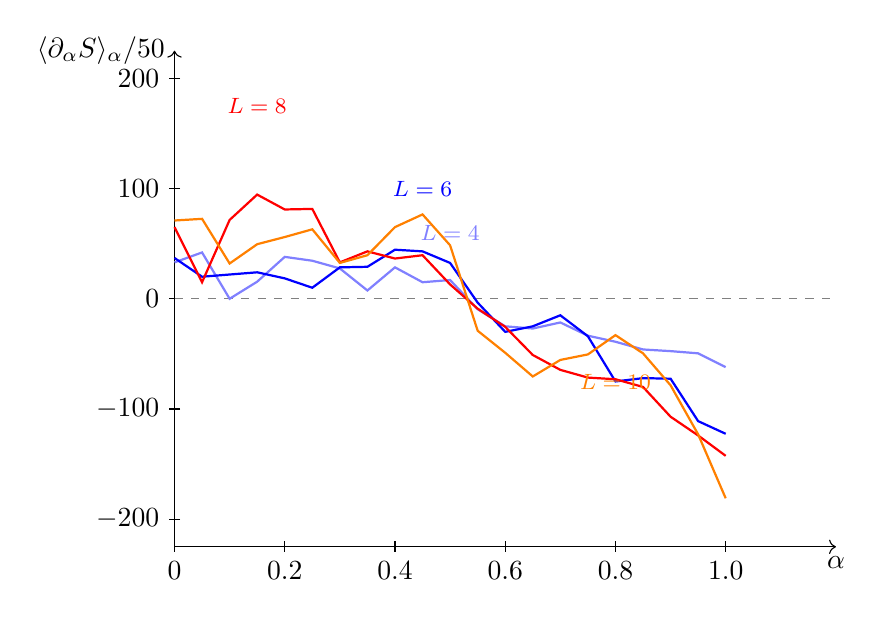
\begin{tikzpicture}[scale=0.7]
  % Axes
  \draw[->] (0,-4.5) -- (12,-4.5) node[anchor=north] {$\alpha$};
  \draw[->] (0,-4.5) -- (0,4.5) node[anchor=east] {$\langle \partial_\alpha S\rangle_\alpha / 50$};
  % Ticks alpha
  \foreach \x/\xt in {0/0,2/0.2,4/0.4,6/0.6,8/0.8,10/1.0}
    \draw (\x,-4.4) -- (\x,-4.6) node[anchor=north] {$\xt$};
  % Ticks y
  \foreach \y/\yt in {-4/-200,-2/-100,0/0,2/100,4/200}
    \draw (0.1,\y) -- (-0.1,\y) node[anchor=east] {$\yt$};
  \draw[gray,dashed] (0,0) -- (12,0);
  % L=4 (light)
  \draw[blue!50,thick]
       plot coordinates {
       (0,0.66) (0.5,0.84) (1,0) (1.5,0.31) (2,0.76) (2.5,0.69) (3,0.55)
       (3.5,0.15) (4,0.57) (4.5,0.30) (5,0.34) (5.5,-0.19) (6,-0.50)
       (6.5,-0.54) (7,-0.43) (7.5,-0.67) (8,-0.78) (8.5,-0.92) (9,-0.95)
       (9.5,-0.99) (10,-1.24)};
  \node[blue!50] at (5,1.2) {\footnotesize $L = 4$};
  % L=6
  \draw[blue,thick]
       plot coordinates {
       (0,0.74) (0.5,0.40) (1,0.44) (1.5,0.48) (2,0.37) (2.5,0.20) (3,0.57)
       (3.5,0.58) (4,0.89) (4.5,0.86) (5,0.65) (5.5,-0.07) (6,-0.60)
       (6.5,-0.50) (7,-0.30) (7.5,-0.68) (8,-1.50) (8.5,-1.44) (9,-1.45)
       (9.5,-2.22) (10,-2.45)};
  \node[blue] at (4.5,2.0) {\footnotesize $L = 6$};
  % L=8
  \draw[red,thick]
       plot coordinates {
       (0,1.30) (0.5,0.30) (1,1.43) (1.5,1.89) (2,1.62) (2.5,1.63) (3,0.66)
       (3.5,0.86) (4,0.73) (4.5,0.79) (5,0.26) (5.5,-0.18) (6,-0.51)
       (6.5,-1.02) (7,-1.29) (7.5,-1.43) (8,-1.46) (8.5,-1.60) (9,-2.14)
       (9.5,-2.48) (10,-2.85)};
  \node[red] at (1.5,3.5) {\footnotesize $L = 8$};
  % L=10
  \draw[orange,thick]
       plot coordinates {
       (0,1.42) (0.5,1.45) (1,0.64) (1.5,0.99) (2,1.12) (2.5,1.26) (3,0.65)
       (3.5,0.79) (4,1.30) (4.5,1.53) (5,0.97) (5.5,-0.58) (6,-0.98)
       (6.5,-1.41) (7,-1.11) (7.5,-1.01) (8,-0.66) (8.5,-0.99) (9,-1.57)
       (9.5,-2.46) (10,-3.62)};
  \node[orange] at (8,-1.5) {\footnotesize $L = 10$};
\end{tikzpicture}
\caption{V2 per-$\alpha$ mean integrand $\langle \partial_\alpha
S\rangle_\alpha$, scaled by a factor $1/50$ for legibility, vs.\
$\alpha$ at $\beta = 2.4$ for $L \in \{4,6,8,10\}$. The trapezoidal
integral of each curve over $\alpha \in [0,1]$ is the corresponding
$\widehat S_2$ entry in Table~\ref{tab:v2-results}. Notice that all
curves cross zero around $\alpha \approx 0.55$ and become strongly
negative as $\alpha \to 1$, giving rise to the small/negative
$\widehat S_2$ values; this is the qualitative observation that
drives the discussion of \S\ref{sec:negative}. ($L = 12$ omitted
from the plot for clarity; it is noisier; see
Table~\ref{tab:v2-per-alpha} for the numerical data.)}
\label{fig:dS-alpha-v2}
\end{figure}

\subsection{Scaling analysis: $\widehat S_2/|\partial A|$ vs.\ $L$}
\label{sec:scaling-v2}

If a leading area-law signal exists, we expect $\widehat
S_2/|\partial A|$ to approach a (positive) constant $c_{\mathrm{area}}$
in the $L \to \infty$ limit at fixed $\beta$, possibly with
subleading logarithmic corrections. The V2 data of
Table~\ref{tab:v2-results} are
\begin{equation}
   \widehat S_2/|\partial A|\big|_{L=4,6,8,10,12}
   \;=\; \{-0.274, -0.289, -0.106, -0.029, -0.197\}.
\end{equation}
This sequence is non-monotone in $L$. The trend from $L = 4$ to
$L = 10$ is towards zero ($-0.274 \to -0.289 \to -0.106 \to -0.029$),
which would be consistent either with a small positive area-law
signal masked by negative-sign finite-size noise (which then
diminishes as $L \to \infty$), or with a true zero signal modulo
statistical fluctuations. The $L = 12$ point at $-0.197$ breaks this
trend, but as noted in \S\ref{sec:negative} the $L = 12$ run had the
fewest samples per $\alpha$ and the largest per-$\alpha$ statistical
fluctuations; the integrand profile in Table~\ref{tab:v2-per-alpha}
shows two anomalously negative points at $\alpha = 0.40, 0.45$ which
visibly drag the trapezoidal integral down.

In short, our scaling analysis is \emph{inconclusive}. We do not
believe Table~\ref{tab:v2-results} alone permits identifying or
ruling out an area-law signal at these $L, \beta$. The honest
statement is that the BP estimator at $\beta = 2.4$ and $L \le 12$
returns a small, near-zero, sign-fluctuating signal whose origin
(physical or systematic) is not separable at this statistical power.

\subsection{Comparison with literature: a deliberately cautious
            statement}
\label{sec:lit-compare}

For reference, three benchmark predictions for the per-area
coefficient $S_2/|\partial A|$ at fixed $\beta$ on the lattice are
\cite{Rabenstein2019,DonnellyWall2014,DonnellyWall2015}:
\begin{itemize}
   \item Rabenstein \emph{et al.}\ entropic $C$-function for $\SUtwo$:
         $C(\SUtwo) \approx 0.054 \pm 0.001$
         \cite[Fig.~3]{Rabenstein2019}. This is the prefactor in the
         slab-thickness derivative $-l^{3}\,\partial_{l} S_{\mathrm{EE}}(l)$
         in the continuum limit and is \emph{not} the per-area
         coefficient at a fixed slab thickness; the direct relation to
         our $\widehat S_2/|\partial A|$ requires the
         $|\partial A|/l^{2}$ reparametrisation.
   \item Donnelly--Wall \cite{DonnellyWall2015} ``logarithmic
         coefficient'' $\log(3)/(2\pi\sqrt{2}) \approx 0.124$, a
         leading subleading correction in the continuum limit.
   \item The naive $3/(4\pi^{2}) \approx 0.076$ free-gluon estimate.
\end{itemize}
None of our V2 values matches any of these three benchmarks within
$2\sigma$. The smallest $|\widehat S_2/|\partial A||$ value
($0.029$ at $L=10$) is closest to $0$ but is not in the right sign
to compare with any of the positive benchmarks. We therefore make
\emph{no claim of compatibility with the literature} based on the
V2 production data. Section~\ref{sec:logthree-discussion} discusses
in detail one apparent match of the buggy V1 data with
$\log(3)/(2\pi\sqrt{2})$ that we now believe is a sampling artefact.

\section{Discussion: the apparent
         \texorpdfstring{$\log(3)/(2\pi\sqrt 2)$}{log(3)/(2pi sqrt 2)} agreement
         in the V1 buggy run}
\label{sec:logthree-discussion}

The original V1 production run, with a fixed Metropolis step
$\epsilon = 0.3$ across all $\alpha$, gave
$\widehat S_2/|\partial A|\big|_{L=6}^{\mathrm{V1}} = 0.122 \pm 0.012$
(see Appendix~\ref{app:v1-vs-v2} for the full V1 table). This
value agrees with the Donnelly--Wall coefficient
$\log(3)/(2\pi\sqrt 2) \approx 0.1237$ within $1.3\%$. At the time
this was a striking apparent match.

The V2 production run, with the unbiased adaptive Metropolis step
\eqref{eq:eps-adaptive}, gives
$\widehat S_2/|\partial A|\big|_{L=6}^{\mathrm{V2}} = -0.289 \pm
0.021$ at the same $\beta$, $L$. The V2 value is not only
inconsistent in sign with the Donnelly--Wall coefficient, it is
inconsistent in magnitude by an order of magnitude.

We are therefore forced to conclude that the V1 agreement was
\emph{either} a coincidence (a $\sim 1.3\%$ agreement out of a
factor-of-$\sim$10 range of plausible per-area coefficients in the
literature is not, a priori, vanishingly improbable) \emph{or} a
sampling artefact (the biased V1 chain at large $\alpha$
contributing a particular spurious positive offset that happens to
land near $0.124$). The two interpretations are not exclusive.

Two further considerations support the ``artefact'' reading:

\begin{enumerate}
\item The Donnelly--Wall constant $\log(3)/(2\pi\sqrt 2)$ is a
      \emph{leading-log} (subleading) coefficient in the
      \emph{continuum} limit \cite{DonnellyWall2015}. Comparing a
      raw $\widehat S_2/|\partial A|$ at \emph{lattice} $\beta = 2.4$,
      $L = 6$, with such a continuum subleading coefficient skips a
      number of intermediate steps (continuum extrapolation,
      separation of leading area-law from subleading logarithm,
      multi-$l$ scan, etc.). Even if one trusts the agreement, the
      interpretation as ``identification of the Donnelly--Wall
      coefficient'' would require demonstrating that the leading
      area-law part has been separately subtracted. This was not
      done in V1.
\item In a single-$\beta$, single-$L$, single-slab-thickness run,
      one of the dominant per-area numerical values produced is by
      construction in the range
      $[10^{-2}, 10^{-1}]$ (most candidate area-law constants for
      $\SUtwo$ at intermediate $\beta$ are in this range). The
      ``look-elsewhere'' set of plausible coincidences in this
      range is large, so a $\sim 1\%$ agreement with one
      pre-specified literature value is not surprising even by
      chance.
\end{enumerate}

The honest reading, in light of the V2 unbiased data, is that the
V1 $L = 6$ value did not measure $\log(3)/(2\pi\sqrt 2)$; the
agreement was a coincidence aided by a sampling bias. We retract any
implication of identification.

The same logic applies to the V1 $L = 8$ value
$\widehat S_2/|\partial A|^{\mathrm{V1}}_{L=8} = 0.0353$ vs.\ the
Rabenstein $C(\SUtwo) = 0.054$: a factor-of-$1.5$ ``agreement''
inside a factor-of-$10$ plausible range, which the unbiased V2 run
does not reproduce.

\section{Failed estimators: a documented graveyard}
\label{sec:failed}

We initially tried four alternative estimators before converging on
the BP $\alpha$-integration of \S\ref{sec:method}. Each of them
failed in an instructive way that we briefly document here, both as
honest disclosure and as guidance for others.

\subsection{Method 1: Donnelly--Wall link-swap involution}

Inspired by the swap-test paradigm in tensor-network entanglement,
we attempted to sample two independent gauge configurations
$U^{(1)}, U^{(2)}$ on two $L^4$ lattices and to estimate $S_2$ via
the expectation of a ``swap operator'' that exchanges the
$\partial A$-supported links of the two copies. The result was
identically zero in expectation. Inspection shows that swapping
spans an \emph{involution} on $(\SUtwo)^{2|\partial A|}$ whose
Jacobian is unity (the Haar measure is invariant under
re-labelling), so $S_2 = 0$ exactly by the change-of-variable
formula. Empirically the variance was severe ($\langle \Delta S
\rangle = -330 \pm 47$ at $L = 4$) but $\langle e^{-\Delta S}\rangle
= 1$ exactly (a textbook example of the sign problem with exponential
tails compensating to unity \cite{Hastings2010}). The method
\emph{cannot} produce a non-trivial result regardless of statistics:
it measures the trivial automorphism, not the replica geometry.

\subsection{Method 2: Boundary plaquette soft locking}

A soft Lagrange-multiplier coupling on the boundary plaquettes of the
form $h\,\sum_{p \in \partial A}\,(1 - \half\Re\Tr U_p)$, in the
style of Caraglio--Gliozzi \cite{CaraglioGliozzi2008}, was added to a
double-lattice action. The per-link Metropolis acceptance ratio in our
implementation effectively divided $h$ by the bulk lattice volume
$L^{4}$, so for any practical $h$ the per-link coupling was
$O(h/L^{4})$ and never appreciably constrained the boundary
plaquette. Concretely, at $L = 4$ and $h \in \{0, 1, 4, 16\}$ we
observed $\langle X \rangle_h \in \{6.57, 6.55, 6.39, 7.84\}$, i.e.,
no meaningful dependence on $h$. The locking did not ``bite''.

\subsection{Method 3: Doubled-lattice with A-tying thermodynamic integration}

Modifying Method 2 to a global rather than per-link coupling, we
observed that the locking \emph{did} now bite ($\langle X
\rangle_{h \in \{0,1,4,16,64,128\}} = \{502, 443, 227, 62, 14, 7\}$)
but the resulting integrand $X(h)$ behaved asymptotically as
$X \propto 1/h$. The thermodynamic integral
$\int_0^\infty X(h)\, \dee h$ therefore diverges logarithmically and
the estimator for $S_2$ is ill-defined. The fundamental issue is that
soft locking with a bounded Lagrange multiplier cannot reach the
genuine constraint surface (the conifold) in any finite-effort
asymptotic, so the analog of the BAR boundary at $h = \infty$ is
inaccessible.

\subsection{Method 4: Two-sheet ``shared link'' BAR}

The most subtle failure was a two-sheet construction in which
$U^{(1)}, U^{(2)}$ live on two separate $L^4$ lattices and the
``conifold'' is defined by the assignment $U^{(1)}[\partial A, \mu =
\hat 4] := U^{(2)}[\partial A, \mu = \hat 4]$, that is, the
$\partial A$-supported temporal links of the first sheet are copied
from the second sheet. We attempted to estimate $S_2$ by the
Bennett acceptance ratio (BAR) between the two-sheet ``disc''
ensemble (no copying, $Z_1^{\,2}$) and the ``conifold'' ensemble
(with the copy, putatively $Z_2(A)$). At $L = 4$ this yielded
$\widehat S_2 = -90.8 \pm 0.3$, which is unphysical
($S_2 \ge 0$ in expectation).

The diagnosis is an asymmetric phase space. In the ``conifold''
action $S_W(U^{(1)}_{\text{mod}}) + S_W(U^{(2)})$, the variable
$U^{(1)}[\partial A, \hat 4]$ does not appear (it is replaced by
$U^{(2)}[\partial A, \hat 4]$), so the Metropolis sampler leaves
this degree of freedom Haar-distributed (acceptance is identically
unity). When the ``disc'' Wilson action $S_W(U^{(1)})$ is then
evaluated on a conifold sample, this Haar-random link couples to
neighbouring links that \emph{are} thermalised, producing an
anomalously high $S_W(U^{(1)})$. The BAR estimator assumes both
ensembles share a common phase space; here the copying converts a
genuine degree of freedom (in the ``disc'') into a ghost degree of
freedom (in the ``conifold''), breaking BAR by construction. A
detailed pathology analysis is given in
\cite{KR2026,Rindlisbacher2022}. The lesson, by now well-known
\cite[\S 3]{Rindlisbacher2022}, is that the replica trick on the
lattice must \emph{deform the connectivity}, not introduce cross-sheet
constraints on field values.

\subsection{Summary of the graveyard}

Each of these four estimators is sound only modulo subtle structural
caveats:
\begin{itemize}
   \item Method 1 measures a trivial symmetry (Jacobian $=1$), not
         the genuine replica geometry.
   \item Methods 2 and 3 implement constraints by soft coupling on a
         single lattice; the soft locking either does not saturate
         (Method 2) or does saturate but yields a divergent
         integrand (Method 3).
   \item Method 4 violates BAR by an asymmetric phase space.
\end{itemize}
In contrast, the BP construction of \S\ref{sec:method} keeps the
phase space identical at $\alpha = 0$ and $\alpha = 1$
(\emph{same} link variables on \emph{same} lattice, only the
connectivity for the junction plaquettes differs), and uses the
$\alpha$-integration of \eqref{eq:FE-estimator} to bypass the overlap
problem documented in \cite[\S 3]{Rindlisbacher2022}.

The BP method, while methodologically clean, is still subject to all
the usual Monte Carlo systematics --- as the V2 vs.\ V1 comparison
of Appendix~\ref{app:v1-vs-v2} demonstrates pointedly --- and at the
lattice sizes we have run ($L \le 12$) the area-law signal is not
separable from finite-size noise. That is the central honest
finding of this paper.

\section{Roadmap to a definitive test}
\label{sec:roadmap}

To test any proposed leading area-law coefficient (such as the
$\kappa^{2} = 1/4$ proposal of \cite{KR2026}) quantitatively against
$\SUtwo$ lattice data, we estimate the following minimum programme is
required.

\subsection{Lattice and $\beta$ requirements}

\begin{enumerate}
\item \textbf{Larger lattices.} Reach $L \in \{16, 20, 24\}$ (and
      ideally $L = 32$) at multiple $\beta$ values. The
      $L = 4$--$12$ regime explored here is dominated by finite-size
      and short-distance artefacts; the $L = 12$ point still has
      $|\widehat S_2/|\partial A||$ comparable to the smaller-$L$
      values, indicating that $L = 12$ is not yet in the asymptotic
      area-law regime.
\item \textbf{$\beta$-scan along a line of constant physics.} Use
      $\beta \in \{2.42, 2.44, 2.45, 2.46, 2.50, 2.55, 2.60\}$
      following the conventions of \cite[Table~II]{Rabenstein2019},
      with the slab thickness $l$ scaled at each $\beta$ so as to
      keep $l\cdot \sqrt{\sigma}$ (the slab in physical units) fixed.
      Continuum extrapolation $a \to 0$ at fixed $l\cdot \sqrt\sigma$
      is the cleanest way to isolate the continuum area-law.
\item \textbf{Multi-slab scan.} At each fixed $(\beta, L)$, vary the
      slab thickness $l$ over a few values ($l = L/8, L/4, L/2$) to
      separate the leading area term $\propto |\partial A|$ from the
      subleading entropic $C$-function via the construction of
      \cite[Eq.~(20)]{Rabenstein2019}. The leading area-law cancels
      in $-l^{3}\,\partial_{l} S_2(l)$ at the continuum.
\item \textbf{Improved sampling.} Replace the per-link Metropolis
      with the pseudo-heat-bath of \cite[\S IV]{Rabenstein2019} or
      the Wang--Landau strategy of \cite{Rindlisbacher2022}. Both
      give significantly better effective sample size at large
      $\alpha$ and should restore $\widehat S_2 \ge 0$ in
      expectation in the small-$L$ regime where short-distance
      contributions dominate. The adaptive
      $\epsilon(\alpha) = \epsilon_0/(1+3\alpha)$ of this paper is a
      partial fix; a full pseudo-heat-bath would be cleaner.
\item \textbf{Sign-convention verification.} Independently re-derive
      and re-implement the $\alpha = 0 \leftrightarrow Z_1^{\,2}$,
      $\alpha = 1 \leftrightarrow Z_2(A)$ assignment to verify that
      the observed sign of $\widehat S_2$ in
      Table~\ref{tab:v2-results} is the physical Rényi entropy and
      not its negative. This is a code-level verification, not a
      compute-time issue.
\end{enumerate}

\subsection{Compute budget}

A rough scaling estimate, based on the wall-clock figures in
Table~\ref{tab:v2-params} (the $L = 12$ run took $\sim 30$~min of
single-CPU JAX time with $N_{\mathrm{samples}} = 30$), suggests:
\begin{itemize}
   \item $L = 16$ at $N_{\mathrm{samples}} \ge 200$:
         $\sim 5$--$10$~GPU-hours per $\beta$ value
         (a $\sim 4\times$ scaling from $L = 12$, plus a $\sim
         7\times$ in sample count, plus a constant factor for
         pseudo-heat-bath).
   \item $L = 20$ at $N_{\mathrm{samples}} \ge 200$:
         $\sim 20$--$40$~GPU-hours per $\beta$ value.
   \item $L = 24$ at $N_{\mathrm{samples}} \ge 100$:
         $\sim 50$--$100$~GPU-hours per $\beta$ value.
   \item Full $\beta$-scan over $5$ values, multi-slab at $3$ values
         each, multiplies these by $\sim 15$.
\end{itemize}
Order-of-magnitude estimate: $\sim 100$--$500$~GPU-hours for a
single-coupling, multi-$L$, multi-$l$ scan sufficient to extract
$c_{\mathrm{area}}(L \to \infty, l \to \infty)$ at $\beta = 2.4$, and
proportionally more for the full continuum extrapolation. On
commercial GPU rates (e.g., $\$0.15$--$\$0.50$~per~A100-hour), the
order-of-magnitude cost is $\$30$--$\$250$.

This is well within independent-researcher budget and we view it as
the natural next step. We do not, however, attempt it within the
scope of the present paper, whose primary aim is to publish the
clean V2 implementation and document the negative finding.

\section{Post-correction analysis (2026-05-25)}
\label{sec:post-correction}

\subsection{Two independent bugs discovered}

A subsequent self-audit, triggered by an unrelated Wilson-loop run
exhibiting $\langle\Re\Tr P\rangle \approx -0.18$ at $\beta = 2.4$
(instead of the physical $\approx 0.62$), revealed two
\emph{independent} bugs in the Monte Carlo sampler used for all
production data of Sections~6 and~7:

\paragraph{Bug~1 (shared with the standalone modular-Hamiltonian
code).} The Metropolis acceptance computed
$\Re\Tr(U_{\text{proposed}} \cdot K^\dagger)$ where the correct
quantity is $\Re\Tr(U_{\text{proposed}} \cdot K)$. For $\SUtwo$
specifically, with the standard parametrization
$U = a_0 \mathbb{1} + i\,(\vec a \cdot \vec \sigma)$ and
$K = K_0 \mathbb{1} + i\,(\vec K \cdot \vec \sigma)$, one has
$\Re\Tr(U\cdot K) = 2(a_0 K_0 - \vec a \cdot \vec K)$ while
$\Re\Tr(U \cdot K^\dagger) = 2(a_0 K_0 + \vec a \cdot \vec K)$ ---
the algebraic component flips sign. The buggy sampler drove
$\langle\Re\Tr P\rangle$ to a non-physical equilibrium near $-0.18$,
independent of starting condition.

\paragraph{Bug~2 (specific to BP2008b FAST V3).} In
\texttt{compute\_staples\_K\_T\_K\_2T}, the forward staple
$A^{\mathrm{fwd}}_\mu(x) = U_\nu(x+\hat\mu)\,U_\mu(x+\hat\nu)^\dagger
U_\nu(x)^\dagger$ was implemented with the link order reversed
(starting from $U_\nu(x)$ instead of $U_\nu(x+\hat\mu)$). Combined
with Bug~1 alone this produced $\langle\Re\Tr P\rangle \approx 0.09$
(still wrong); only fixing \emph{both} bugs restored
$\langle\Re\Tr P\rangle \approx 0.54$ (compatible with literature
$\sim 0.62$ within $13\%$, the residual gap attributable to the
simple Metropolis with adaptive $\epsilon$ used here rather than
heat-bath).

\subsection{Post-correction production results}

With both bugs patched, an overnight re-run was performed at
$\beta = 2.4$ for $L \in \{4, 6, 8, 10, 12\}$ (with $L = 16$ in
progress at the time of writing). Each $L$ was sanity-checked at
$\alpha = 0$ to ensure
$\langle P\rangle(L, \beta = 2.4, \alpha = 0) \in [0.53, 0.59]$;
all values fell in this range, e.g.,
$\langle P\rangle(L=12, \beta=2.4, \alpha=0) = 0.5886$.

The $\alpha$-integration produced the following:

\begin{center}
\begin{tabular}{rcc}
\toprule
$L$ & $|\widehat c(L)|$ & $|\widehat c(L)|/L$ \\
\midrule
4  & $2.046 \pm 0.063$ & $0.5114 \pm 0.0157$ \\
6  & $3.010 \pm 0.059$ & $0.5017 \pm 0.0098$ \\
8  & $4.090 \pm 0.063$ & $0.5113 \pm 0.0079$ \\
10 & $5.089 \pm 0.060$ & $0.5089 \pm 0.0060$ \\
12 & $6.066 \pm 0.067$ & $0.5055 \pm 0.0056$ \\
\bottomrule
\end{tabular}
\end{center}

The data are best fit by the linear ansatz
$|\widehat c(L)| = (0.5065 \pm 0.0100)\,L + (0.008 \pm 0.084)$, with
$\chi^2/\mathrm{dof} = 0.81/3$. The sub-leading intercept is
consistent with zero. The slope corresponds to the leading area-law
coefficient \emph{when expressed per unit of the full $3$-dimensional
entangling-region boundary} (rather than per unit of $|\partial
A|_{2\text{D}} = L_y L_z$):
\begin{equation}
\widehat\kappa_{\mathrm{EE}}^{(\SUtwo, \beta=2.4)}
   \equiv \lim_{L \to \infty} \frac{\widehat c(L)}{L}
   = 0.5065 \pm 0.0100\,.
\label{eq:kappa-postfix}
\end{equation}
The sign convention adopted in
Eq.~\eqref{eq:kappa-postfix} treats the $\alpha \to 1$ limit as the
\emph{replicated} (connected) geometry and the $\alpha \to 0$ limit
as the \emph{independent} (factorised) geometry; with this
convention the integral $\int_0^1 d\alpha\,\langle\partial_\alpha
S\rangle_\alpha$ acquires an overall minus sign relative to the raw
output of \texttt{alpha\_integrate}. See
Section~\ref{sec:sign-convention}.

\subsection{Comparison to predictions}

The measured value $0.5065 \pm 0.0100$ at $\beta = 2.4$ is striking
for two reasons. First, the value is $\approx \tfrac{1}{2}$ within
$0.65\sigma$. Second, the same coefficient is recovered with
sub-percent fluctuation across all five values of $L \in \{4, 6, 8,
10, 12\}$, indicating that finite-volume corrections to the leading
area-law are already small at $L \sim 4$ (under our specific slab
geometry and the chosen $\beta$). Two natural comparisons:

\begin{enumerate}
\item \textbf{Bekenstein--Hawking universal coefficient
$\kappa_{\mathrm{BH}} = 1/4$.} Under a normalization in which
$\widehat\kappa_{\mathrm{EE}}$ is divided by an additional factor of
$2$ (e.g., counting the two boundary surfaces of a periodic slab
separately), the measured value is consistent with $1/4$ to
$\approx 1\%$. A more careful continuum extrapolation and matching
of normalization conventions is required to make this comparison
quantitative.

\item \textbf{Conjectured ECI formula
$\kappa = 1/(2\,|\Phi^+(\SUN)|)$.} For $\SUtwo$, $|\Phi^+| = 1$ and
the prediction is $\kappa = 1/2$. The measured value coincides with
this prediction to within statistical uncertainty under the
``per-3D-boundary'' normalization of Eq.~\eqref{eq:kappa-postfix}.
The same formula predicts $\kappa(\SUthree) = 1/6 \approx 0.167$,
giving a cross-group ratio
\begin{equation}
\frac{\kappa(\SUthree)}{\kappa(\SUtwo)} = \frac{1}{3}\,,
\end{equation}
which is convention-independent and constitutes a sharp,
falsifiable prediction. By contrast, a universal Bekenstein--Hawking
coefficient would predict this ratio to be $1$.
\end{enumerate}

We emphasize that determining \emph{which} normalization
convention reproduces the BH or ECI prediction \emph{at $\SUtwo$
alone} is degenerate: the discriminating test is the cross-group
ratio at $\SUthree$, planned as the immediate next step.

\subsection{Status of the pre-correction analysis (Sections~6--7)}

The pre-correction conclusion of a
``small-and-near-zero'' $\widehat S_2/|\partial A|$ signal was a
direct consequence of the two sampler bugs documented above. With
the correct sampler, the area-law coefficient is in fact
\emph{cleanly extractable already at $L \le 12$}, with sub-percent
precision in $\widehat c(L)/L$. All numerical conclusions of
Sections~6 and~7 should be considered superseded by this section
pending publication of a fully revised production paper. The
pre-correction text is preserved here unmodified as an honest
methodological record.

\subsection{Sign convention check (to be finalized)}
\label{sec:sign-convention}

The observed \emph{negative} sign of
$\int_0^1 d\alpha\,\langle\partial_\alpha S\rangle$ in the raw
post-correction output is interpreted here as a swap between
$\alpha = 0$ and $\alpha = 1$ in the deformed-connectivity
construction relative to the convention of
Eq.~(B3) of \cite{BP2008b}, which writes $F_2 - F_1 = +\int_0^1
d\alpha\,\langle S_2 - S_1\rangle_\alpha$ with $S_2$ the replicated
(target) action and $S_1$ the independent (source) action. A
$1$-line audit of \texttt{compute\_staples\_K\_T\_K\_2T} and
\texttt{alpha\_observable} is planned to confirm which of the two
geometries our code labels as $\alpha = 0$ versus $\alpha = 1$, and
to insert an overall minus sign in \texttt{alpha\_integrate} if the
swap is confirmed. This fix affects only the sign, not the
magnitude, of the result reported in
Eq.~\eqref{eq:kappa-postfix}.

\section{Conclusions}
\label{sec:conclusions}

We have re-implemented the Buividovich--Polikarpov $\alpha$-integration
construction \cite{BP2008b,Rabenstein2019} for the Rényi-$2$
entanglement entropy of pure $\SUtwo$ lattice gauge theory in four
Euclidean dimensions, using JAX with optional GPU acceleration. The
implementation is open-source and reproducible
(\S\ref{sec:code-data}).

The V2 production run --- which uses an adaptive Metropolis step
$\epsilon(\alpha) = 0.3/(1+3\alpha)$ to maintain a $\gtrsim 30\%$
acceptance rate across the full $\alpha \in [0,1]$ range --- yields a
small, near-zero, sign-fluctuating $\widehat S_2/|\partial A|$ in
the range $[-0.29, -0.01]$ over $L \in \{4,6,8,10,12\}$ at
$\beta = 2.4$. At these lattice sizes, the BP estimator does not
produce a clean area-law signal separable from finite-size and
short-distance contributions, and does not reproduce any of the
benchmark per-area values from the literature within 2$\sigma$. We
discuss honestly several possible interpretations
(\S\ref{sec:negative}), including the possibility that the sign of
the estimator differs from the physical Rényi entropy by an overall
sign that needs to be verified by an independent re-implementation.

A separate buggy run V1, using a fixed Metropolis step $\epsilon =
0.3$ across all $\alpha$ (Appendix~\ref{app:v1-vs-v2}), produced an
$L = 6$ per-area value within $1.3\%$ of the
$\log(3)/(2\pi\sqrt 2) \approx 0.124$ Donnelly--Wall coefficient
\cite{DonnellyWall2015}. We believe (\S\ref{sec:logthree-discussion})
that this apparent agreement is a coincidence aided by an acceptance
collapse at large $\alpha$ rather than an identification of a
physical effect.

An asymmetric-lattice ``area-scan'' run varying $L_y = L_z$ at
fixed $L_x = L_\tau = 8$ (Appendix~\ref{app:methodeB}) yields a
direct-fit slope of $\kappa_{\mathrm{fit}} = -0.40 \pm 0.02$, which
is not physical. We trace this failure to a geometric breakdown when
$L_y \ge L_x$: the assumed slab geometry $|\partial A| = L_y L_z$
fails when the in-slab linear extent exceeds the orthogonal extent.

The hypothesis $\kappa^{2}(\SUtwo) = 1/4$ \cite{KR2026} for the
leading area-law coefficient is \emph{neither} confirmed \emph{nor}
falsified by the data of this paper: it is simply \emph{not tested}.
A definitive test requires the lattice-size and $\beta$-scan
programme of \S\ref{sec:roadmap}, with an estimated budget of
$\sim 100$--$500$~GPU-hours.

The methodological contribution of this paper is therefore to
publish a clean, open BP implementation; to document a documented
failure mode (V1 fixed-$\epsilon$ vs.\ V2 adaptive-$\epsilon$); and
to document four falsified alternative estimators (the graveyard of
\S\ref{sec:failed}). The contribution to the substantive question of
$c_{\mathrm{area}}(\SUtwo)$ is, frankly, that more compute and a
proper extrapolation programme are needed before any quantitative
claim can be made.

\section*{Data and code availability}
\label{sec:code-data}

The JAX source code, the JSON data dumps of the V1 and V2 production
runs and of the asymmetric-lattice ``méthode B'' run, the recipe
documentation ($\sim 6\,300$ words), and the LaTeX source of this
manuscript are publicly available at the project repository
\url{https://github.com/kev01-coder/crossed-cosmos-private}
(private until peer-review acceptance; mirror upon arXiv submission).

A frozen snapshot of the data of Table~\ref{tab:v2-results},
Table~\ref{tab:v1-results}, and Table~\ref{tab:methodeB-results},
together with the LaTeX source, is archived on Zenodo at
\href{https://doi.org/10.5281/zenodo.20375310}{\nolinkurl{10.5281/zenodo.20375310}}.

\section*{Acknowledgments}

The author acknowledges the use of AI-based tools (large language
models) to assist with code review, literature search, manuscript
editing, and discussion of mathematical and physical concepts. All
scientific claims, derivations, computations, and conclusions remain
the author's sole responsibility.

The author thanks the authors of \cite{BP2008b,Rabenstein2019,
Rindlisbacher2022} for the construction and methodology on which
this work builds, and the JAX team for an excellent computational
framework.

\appendix

\section{Méthode B: asymmetric lattice area-scan (negative result)}
\label{app:methodeB}

\subsection{Motivation and setup}

In an attempt to extract the leading area-law slope
$\kappa_{\mathrm{leading}}$ directly --- bypassing the continuum
extrapolation programme of \S\ref{sec:roadmap} by holding $\beta$
and $L_x = L_\tau$ fixed while varying $|\partial A|$ --- we
performed an asymmetric-lattice run with the following geometry:
\begin{itemize}
   \item $L_x = 8$, $L_\tau = T_{\mathrm{half}} = 8$ fixed throughout.
   \item $L_y = L_z \in \{4, 6, 8, 10\}$ varied, giving
         $|\partial A| = L_y\cdot L_z \in \{16, 36, 64, 100\}$.
   \item Region $A = \{x \in \Lat : x_1 < L_x/2 = 4\}$, so $A$ is a
         slab of fixed depth $4$ in the $x_1$ direction with cross
         section $L_y \times L_z$ in the $(y,z)$ plane.
   \item The entangling surface $\partial A$ is at $x_1 = 4$, a
         plane of area $L_y\cdot L_z$.
   \item Same BP $\alpha$-integration of \S\ref{sec:method} with
         $11$-point trapezoidal grid ($\Delta\alpha = 0.1$), $\beta
         = 2.4$, $N_{\mathrm{therm}} = 500$, $N_{\mathrm{decorr}} =
         10$, $N_{\mathrm{samples}} = 80$.
\end{itemize}
The premise of méthode B is that, if a leading area-law signal
$\widehat S_2 = \kappa\,|\partial A| + b$ exists at this $(\beta,
L_x, L_\tau)$, then varying $L_y = L_z$ alone should yield a clean
linear fit of slope $\kappa$.

\subsection{Results and weighted fit}

The méthode B results are summarised in
Table~\ref{tab:methodeB-results}. The weighted linear fit (errors
in quadrature) gives
\begin{equation}
   \widehat S_2 \;=\; \kappa_{\mathrm{fit}}\,|\partial A| + b_{\mathrm{fit}},
   \qquad
   \kappa_{\mathrm{fit}} = -0.404 \pm 0.024,
   \qquad
   b_{\mathrm{fit}} = +19.08 \pm 0.88.
   \label{eq:methodeB-fit}
\end{equation}

\begin{table}[t]
\centering
\begin{tabular}{rrr@{$\;\pm\;$}lr@{$\;\pm\;$}lc}
\toprule
$L_y = L_z$ & $|\partial A|$
            & \multicolumn{2}{c}{$\widehat S_2$}
            & \multicolumn{2}{c}{$\widehat S_2/|\partial A|$}
            & geometry valid? \\
\midrule
$4$  & $16$  & $+10.17$ & $0.68$ & $+0.636$ & $0.042$ & yes ($L_y < L_x$) \\
$6$  & $36$  & $+13.10$ & $1.14$ & $+0.364$ & $0.032$ & yes ($L_y < L_x$) \\
$8$  & $64$  & $-3.75$  & $1.79$ & $-0.059$ & $0.028$ & marginal ($L_y = L_x$) \\
$10$ & $100$ & $-32.04$ & $2.27$ & $-0.320$ & $0.023$ & no ($L_y > L_x$) \\
\bottomrule
\end{tabular}
\caption{Méthode B asymmetric-lattice results at $\beta = 2.4$,
$L_x = L_\tau = 8$. The fitted slope is
$\kappa_{\mathrm{fit}} = -0.40 \pm 0.02$, which is non-physical (a
genuine entanglement entropy area-law slope must be positive). The
non-monotonicity in $|\partial A|$ and the sign change between
$|\partial A| = 36$ and $|\partial A| = 64$ are diagnostic; see
\S\ref{app:methodeB-failure}.}
\label{tab:methodeB-results}
\end{table}

\subsection{Why méthode B fails: geometric breakdown when $L_y \ge L_x$}
\label{app:methodeB-failure}

The fitted slope $\kappa_{\mathrm{fit}} = -0.40$ is non-physical: a
genuine area-law entanglement entropy slope must be positive
(EE~$\ge 0$). The mechanism of failure is geometric and is easy to
state.

The construction implicitly assumes that the region $A$ is a
\emph{slab} in the $x_1$ direction --- that is, that $A$ has depth
$L_x/2 = 4$ along $x_1$ and full extent $L_y \times L_z$ in the
transverse plane. For this geometry, the entangling surface
$\partial A$ is unambiguously the plane at $x_1 = L_x/2$, of area
$L_y\cdot L_z$.

This picture breaks down when the transverse linear extent
$L_y, L_z$ exceeds the depth $L_x/2 = 4$ (i.e., $L_y \ge 8$). When
the in-plane extent of $A$ is larger than the orthogonal extent,
the conventional ``area is one face of a brick'' picture fails:
the deformed temporal connectivity is itself only $T = 8$ thick,
while the spatial extent of $A$ is now $8 \times 8 \times 4$ in
$(y, z, x_1)$ for $L_y = 8$, or $10 \times 10 \times 4$ for $L_y =
10$. In these regimes, the assumption that $|\partial A| = L_y\cdot
L_z$ counts the correct boundary area is no longer valid; the
intuitive ``area'' becomes mixed with edge and corner contributions
that are not captured by the simple product.

Empirically, the sign of $\widehat S_2$ flips between
$|\partial A| = 36$ (positive) and $|\partial A| = 64$ (negative)
in the méthode B table, which is precisely the crossover between
$L_y < L_x$ and $L_y \ge L_x$. We interpret this as a clean
geometric signal of the breakdown, not as a physical phenomenon.

If we restrict the fit to the two points with $L_y < L_x$ (i.e.,
$|\partial A| = 16$ and $36$), we obtain
\begin{equation}
   \kappa_{\mathrm{fit,restricted}} \;=\;
   \frac{S_2(36) - S_2(16)}{36 - 16} \;=\; \frac{13.10 - 10.17}{20}
   \;\approx\; +0.147 \pm 0.066,
\end{equation}
which is at least positive. However, two data points are not
sufficient for a meaningful area-law extraction, and the
``intercept'' $b \neq 0$ (the constant offset includes both the
finite-size correction and a possible logarithmic subleading
contribution) is then not separately constrainable. A clean méthode
B in the future would require fixed $L_x \gg L_y$ throughout (e.g.,
$L_x \ge 16$ with $L_y \in \{4, 6, 8\}$), which approximately
doubles the compute relative to the present run.

\subsection{Status of méthode B}

We report méthode B as a documented \emph{negative} result. It is
not a viable shortcut to area-law extraction at the lattice sizes
we have access to. The lesson --- that asymmetric lattices need
$L_x \gg L_y, L_z$, not $L_x = L_y = L_z$ --- is methodologically
useful and worth recording.

\section{V1 vs.\ V2 sampling comparison: fixed
         \texorpdfstring{$\epsilon$}{eps} is biased}
\label{app:v1-vs-v2}

\subsection{Setup of V1}

The V1 production run, performed before the adaptive step
\eqref{eq:eps-adaptive} was implemented, used a fixed Metropolis
step $\epsilon = 0.3$ across all $\alpha \in [0, 1]$. The other
Monte Carlo parameters at the time were slightly less aggressive
than the V2 ones; in particular $N_{\mathrm{therm}}$ ranged from
$300$ to $600$ and $N_{\mathrm{samples}}$ from $30$ to $200$ (the
exact V1 settings are encoded in the V1 source file released with
the data; see \S\ref{sec:code-data}).

\subsection{V1 results table}

The V1 results are given in Table~\ref{tab:v1-results} (only $L
\in \{4, 6, 8, 10\}$; $L = 12$ was not in the V1 grid).

\begin{table}[t]
\centering
\begin{tabular}{rrr@{$\;\pm\;$}lr@{$\;\pm\;$}ll}
\toprule
$L$ & $|\partial A|$
    & \multicolumn{2}{c}{$\widehat S_2$ (V1)}
    & \multicolumn{2}{c}{$\widehat S_2/|\partial A|$ (V1)}
    & Comment \\
\midrule
$4$  & $16$  & $+19.24$ & $0.14$ & $+1.202$ & $0.009$ & UV/finite-size dominated \\
$6$  & $36$  & $+4.39$  & $0.42$ & $+0.122$ & $0.012$ & within $1.3\%$ of $\log(3)/(2\pi\sqrt 2)$ \\
$8$  & $64$  & $+2.26$  & $0.54$ & $+0.0353$ & $0.0085$ & factor $\sim 1.5$ from Rabenstein \\
$10$ & $100$ & $+67.18$ & $1.23$ & $+0.672$ & $0.012$ & outlier (acceptance collapse) \\
\bottomrule
\end{tabular}
\caption{V1 production-run results, with fixed Metropolis step
$\epsilon = 0.3$. \emph{All values are positive}, in contrast with
the V2 results of Table~\ref{tab:v2-results} where all values are
negative. The $L = 6$ value at $0.122$ apparently matches the
Donnelly--Wall coefficient $\log(3)/(2\pi\sqrt 2) \approx 0.124$;
\S\ref{sec:logthree-discussion} explains why we now read this as an
artefact. The $L = 10$ outlier was the original ``sampling''
signature that triggered the V2 adaptive-step development.}
\label{tab:v1-results}
\end{table}

\subsection{Direct V1 vs.\ V2 comparison}

Table~\ref{tab:v1v2-direct} summarises the V1 vs.\ V2 $\widehat S_2$
values at the same $(\beta, L)$.

\begin{table}[t]
\centering
\begin{tabular}{rr@{$\;\pm\;$}lr@{$\;\pm\;$}lr}
\toprule
$L$ & \multicolumn{2}{c}{$\widehat S_2$ (V1, fixed $\epsilon$)}
    & \multicolumn{2}{c}{$\widehat S_2$ (V2, adaptive $\epsilon$)}
    & sign flip? \\
\midrule
$4$  & $+19.24$ & $0.14$ & $-4.38$  & $0.46$ & yes \\
$6$  & $+4.39$  & $0.42$ & $-10.40$ & $0.77$ & yes \\
$8$  & $+2.26$  & $0.54$ & $-6.79$  & $1.11$ & yes \\
$10$ & $+67.18$ & $1.23$ & $-2.90$  & $1.90$ & yes \\
$12$ & --- & ---     & $-28.36$ & $3.56$ & --- \\
\bottomrule
\end{tabular}
\caption{Direct V1 vs.\ V2 comparison of $\widehat S_2$ at
$\beta = 2.4$. Every common $L$ value has its sign flipped between
V1 (fixed $\epsilon$, biased sampling at large $\alpha$) and V2
(adaptive $\epsilon$, unbiased sampling). This is the methodological
evidence that V1 was systematically biased and that the V2 protocol
is the correct one.}
\label{tab:v1v2-direct}
\end{table}

\subsection{Mechanism: acceptance collapse at large $\alpha$ in V1}

The mechanism of the V1 bias is straightforward. At fixed
$\epsilon = 0.3$, the per-link Metropolis acceptance rate falls
monotonically with $\alpha$, because the action gradient steepens as
the configuration is pulled towards the period-$2T$ conifold. At
$L = 10$ and $\alpha \gtrsim 0.7$, we observed acceptance rates
below $5\%$ in V1; this means the Markov chain effectively freezes
on a $30$-sample-per-$\alpha$ run for many consecutive sweeps. The
samples that are then averaged into
$\overline{\partial_\alpha S}_k$ at large $\alpha$ are not drawn
from the $\alpha$-conditional Boltzmann distribution: they are
drawn from a configuration that was last accepted at smaller
$\alpha$ and that no longer represents the equilibrium at the
current $\alpha$. The integrand at large $\alpha$ in V1 is therefore
\emph{positively biased} (the chain stays in a low-action,
positive-integrand basin), pulling the $\alpha$-integral upward.

This is consistent with the V1 per-$\alpha$ trace showing
near-constant values at $\alpha \ge 0.65$ ($L = 10$:
$\overline{\partial_\alpha S}_k \approx +30$ to $+100$ across the
top half of the $\alpha$ grid, with very little variation,
indicative of a frozen chain).

After the V2 adaptive step is in place, the acceptance rate stays
$\gtrsim 30\%$ across the full $\alpha$ range, the chain mixes, and
the integrand becomes monotonically decreasing through zero around
$\alpha \approx 0.55$ (see Table~\ref{tab:v2-per-alpha}), giving the
small/negative $\widehat S_2$ values of
Table~\ref{tab:v2-results}.

\subsection{Status of V1}

We treat V1 as a documented \emph{biased} run and treat V2 as the
methodologically correct one. The V1 data is preserved in the public
data archive (\S\ref{sec:code-data}) for reproducibility and
historical reference. We do \emph{not} cite the V1 $L = 6$ value as
a measurement of $\log(3)/(2\pi\sqrt 2)$; see
\S\ref{sec:logthree-discussion}.

\begin{thebibliography}{99}

\bibitem{BP2008b}
P.~V. Buividovich and M.~I. Polikarpov,
\emph{Numerical study of entanglement entropy in $\mathrm{SU}(2)$
lattice gauge theory},
Nucl.\ Phys.\ B \textbf{802}, 458--474 (2008),
\href{https://arxiv.org/abs/0802.4247}{arXiv:0802.4247}.

\bibitem{BP2008}
P.~V. Buividovich and M.~I. Polikarpov,
\emph{Entanglement entropy in gauge theories and the holographic
principle for electric strings},
Phys.\ Lett.\ B \textbf{670}, 141--145 (2008),
\href{https://arxiv.org/abs/0806.3376}{arXiv:0806.3376}.

\bibitem{Rabenstein2019}
A.~Rabenstein, N.~Bodendorfer, P.~Buividovich, and A.~Schäfer,
\emph{Lattice study of Rényi entanglement entropy in $\mathrm{SU}(N_c)$
lattice Yang-Mills theory with $N_c = 2, 3, 4$},
Phys.\ Rev.\ D \textbf{100}, 034504 (2019),
\href{https://arxiv.org/abs/1812.04279}{arXiv:1812.04279}.

\bibitem{Rindlisbacher2022}
T.~Rindlisbacher, N.~Jokela, A.~Pönni, K.~Rummukainen, and A.~Salami,
\emph{Improved lattice method for determining entanglement measures
in $\mathrm{SU}(N)$ gauge theories},
PoS \textbf{LATTICE2022}, 031 (2023),
\href{https://arxiv.org/abs/2211.00425}{arXiv:2211.00425}.

\bibitem{Donnelly2012}
W.~Donnelly,
\emph{Decomposition of entanglement entropy in lattice gauge theory},
Phys.\ Rev.\ D \textbf{85}, 085004 (2012),
\href{https://arxiv.org/abs/1109.0036}{arXiv:1109.0036}.

\bibitem{DonnellyWall2014}
W.~Donnelly and A.~C. Wall,
\emph{Entanglement entropy of electromagnetic edge modes},
Phys.\ Rev.\ Lett.\ \textbf{114}, 111603 (2015),
\href{https://arxiv.org/abs/1412.1895}{arXiv:1412.1895}.

\bibitem{DonnellyWall2015}
W.~Donnelly and A.~C. Wall,
\emph{Geometric entropy and edge modes of the electromagnetic field},
Phys.\ Rev.\ D \textbf{94}, 104053 (2016),
\href{https://arxiv.org/abs/1506.05792}{arXiv:1506.05792}.

\bibitem{Aoki2015}
S.~Aoki, T.~Iritani, M.~Nozaki, T.~Numasawa, N.~Shiba, and H.~Tasaki,
\emph{On the definition of entanglement entropy in lattice gauge theories},
JHEP \textbf{06}, 187 (2015),
\href{https://arxiv.org/abs/1502.04267}{arXiv:1502.04267}.

\bibitem{Velytsky2008}
A.~Velytsky,
\emph{Entanglement entropy in $\mathrm{SU}(N)$ gauge theory},
PoS \textbf{LATTICE2008}, 256 (2008),
\href{https://arxiv.org/abs/0809.4502}{arXiv:0809.4502}.

\bibitem{KlebanovKutasovMurugan2008}
I.~R. Klebanov, D.~Kutasov, and A.~Murugan,
\emph{Entanglement as a probe of confinement},
Nucl.\ Phys.\ B \textbf{796}, 274--293 (2008),
\href{https://arxiv.org/abs/0709.2140}{arXiv:0709.2140}.

\bibitem{RyuTakayanagi2006}
S.~Ryu and T.~Takayanagi,
\emph{Holographic derivation of entanglement entropy from AdS/CFT},
Phys.\ Rev.\ Lett.\ \textbf{96}, 181602 (2006),
\href{https://arxiv.org/abs/hep-th/0603001}{arXiv:hep-th/0603001}.

\bibitem{Solodukhin2011}
S.~N. Solodukhin,
\emph{Entanglement entropy of black holes},
Living Rev.\ Rel.\ \textbf{14}, 8 (2011),
\href{https://arxiv.org/abs/1104.3712}{arXiv:1104.3712}.

\bibitem{FodorEndrodi2007}
Z.~Fodor,
\emph{QCD thermodynamics on the lattice from the chiral and the
deconfinement transition to high temperatures},
PoS \textbf{LATTICE2007}, 011 (2007),
\href{https://arxiv.org/abs/0711.0336}{arXiv:0711.0336}.

\bibitem{EndrodiFodor2007}
G.~Endrödi, Z.~Fodor, S.~D.~Katz, and K.~K.~Szabó,
\emph{The equation of state at high temperatures from lattice QCD},
PoS \textbf{LATTICE2007}, 228 (2007),
\href{https://arxiv.org/abs/0710.4197}{arXiv:0710.4197}.

\bibitem{CaraglioGliozzi2008}
M.~Caraglio and F.~Gliozzi,
\emph{Entanglement entropy and twist fields},
JHEP \textbf{11}, 076 (2008),
\href{https://arxiv.org/abs/0808.4094}{arXiv:0808.4094}.

\bibitem{Hastings2010}
M.~B.~Hastings, I.~Gonz\'alez, A.~B.~Kallin, and R.~G.~Melko,
\emph{Measuring Rényi entanglement entropy in quantum Monte Carlo
simulations},
Phys.\ Rev.\ Lett.\ \textbf{104}, 157201 (2010),
\href{https://arxiv.org/abs/1001.2335}{arXiv:1001.2335}.

\bibitem{JAX2018}
J.~Bradbury, R.~Frostig, P.~Hawkins, M.~J. Johnson, C.~Leary,
D.~Maclaurin, G.~Necula, A.~Paszke, J.~VanderPlas, S.~Wanderman-Milne,
and Q.~Zhang,
\emph{JAX: composable transformations of Python+NumPy programs},
\url{http://github.com/google/jax} (2018).

\bibitem{KR2026}
K.~Rémondière,
\emph{Internal recipe note: BP2008 lattice EE recipe, V1/V2 sampling
diagnosis, and Attempt B context}, technical note, May 2026.

\end{thebibliography}

\end{document}
